\documentclass[1p]{elsarticle_modified}
%\bibliographystyle{elsarticle-num}

%\usepackage[colorlinks]{hyperref}
%\usepackage{abbrmath_seonhwa} %\Abb, \Ascr, \Acal ,\Abf, \Afrak
\usepackage{amsfonts}
\usepackage{amssymb}
\usepackage{amsmath}
\usepackage{amsthm}
\usepackage{scalefnt}
\usepackage{amsbsy}
\usepackage{kotex}
\usepackage{caption}
\usepackage{subfig}
\usepackage{color}
\usepackage{graphicx}
\usepackage{xcolor} %% white, black, red, green, blue, cyan, magenta, yellow
\usepackage{float}
\usepackage{setspace}
\usepackage{hyperref}

\usepackage{tikz}
\usetikzlibrary{arrows}

\usepackage{multirow}
\usepackage{array} % fixed length table
\usepackage{hhline}

%%%%%%%%%%%%%%%%%%%%%
\makeatletter
\renewcommand*\env@matrix[1][\arraystretch]{%
	\edef\arraystretch{#1}%
	\hskip -\arraycolsep
	\let\@ifnextchar\new@ifnextchar
	\array{*\c@MaxMatrixCols c}}
\makeatother %https://tex.stackexchange.com/questions/14071/how-can-i-increase-the-line-spacing-in-a-matrix
%%%%%%%%%%%%%%%

\usepackage[normalem]{ulem}

\newcommand{\msout}[1]{\ifmmode\text{\sout{\ensuremath{#1}}}\else\sout{#1}\fi}
%SOURCE: \msout is \stkout macro in https://tex.stackexchange.com/questions/20609/strikeout-in-math-mode

\newcommand{\cancel}[1]{
	\ifmmode
	{\color{red}\msout{#1}}
	\else
	{\color{red}\sout{#1}}
	\fi
}

\newcommand{\add}[1]{
	{\color{blue}\uwave{#1}}
}

\newcommand{\replace}[2]{
	\ifmmode
	{\color{red}\msout{#1}}{\color{blue}\uwave{#2}}
	\else
	{\color{red}\sout{#1}}{\color{blue}\uwave{#2}}
	\fi
}

\newcommand{\Sol}{\mathcal{S}} %segment
\newcommand{\D}{D} %diagram
\newcommand{\A}{\mathcal{A}} %arc


%%%%%%%%%%%%%%%%%%%%%%%%%%%%%5 test

\def\sl{\operatorname{\textup{SL}}(2,\Cbb)}
\def\psl{\operatorname{\textup{PSL}}(2,\Cbb)}
\def\quan{\mkern 1mu \triangleright \mkern 1mu}

\theoremstyle{definition}
\newtheorem{thm}{Theorem}[section]
\newtheorem{prop}[thm]{Proposition}
\newtheorem{lem}[thm]{Lemma}
\newtheorem{ques}[thm]{Question}
\newtheorem{cor}[thm]{Corollary}
\newtheorem{defn}[thm]{Definition}
\newtheorem{exam}[thm]{Example}
\newtheorem{rmk}[thm]{Remark}
\newtheorem{alg}[thm]{Algorithm}

\newcommand{\I}{\sqrt{-1}}
\begin{document}

%\begin{frontmatter}
%
%\title{Boundary parabolic representations of knots up to 8 crossings}
%
%%% Group authors per affiliation:
%\author{Yunhi Cho} 
%\address{Department of Mathematics, University of Seoul, Seoul, Korea}
%\ead{yhcho@uos.ac.kr}
%
%
%\author{Seonhwa Kim} %\fnref{s_kim}}
%\address{Center for Geometry and Physics, Institute for Basic Science, Pohang, 37673, Korea}
%\ead{ryeona17@ibs.re.kr}
%
%\author{Hyuk Kim}
%\address{Department of Mathematical Sciences, Seoul National University, Seoul 08826, Korea}
%\ead{hyukkim@snu.ac.kr}
%
%\author{Seokbeom Yoon}
%\address{Department of Mathematical Sciences, Seoul National University, Seoul, 08826,  Korea}
%\ead{sbyoon15@snu.ac.kr}
%
%\begin{abstract}
%We find all boundary parabolic representation of knots up to 8 crossings.
%
%\end{abstract}
%\begin{keyword}
%    \MSC[2010] 57M25 
%\end{keyword}
%
%\end{frontmatter}

%\linenumbers
%\tableofcontents
%
\newcommand\colored[1]{\textcolor{white}{\rule[-0.35ex]{0.8em}{1.4ex}}\kern-0.8em\color{red} #1}%
%\newcommand\colored[1]{\textcolor{white}{ #1}\kern-2.17ex	\textcolor{white}{ #1}\kern-1.81ex	\textcolor{white}{ #1}\kern-2.15ex\color{red}#1	}

{\Large $\underline{11a_{34}~(K11a_{34})}$}

\setlength{\tabcolsep}{10pt}
\renewcommand{\arraystretch}{1.6}
\vspace{1cm}\begin{tabular}{m{100pt}>{\centering\arraybackslash}m{274pt}}
\multirow{5}{120pt}{
	\centering
	\includegraphics[width=112pt]{../../../GIT/diagram.site/Diagrams/png/283_11a_34.png}\\
\ \ \ A knot diagram\footnotemark}&
\allowdisplaybreaks
\textbf{Linearized knot diagam} \\
\cline{2-2}
 &
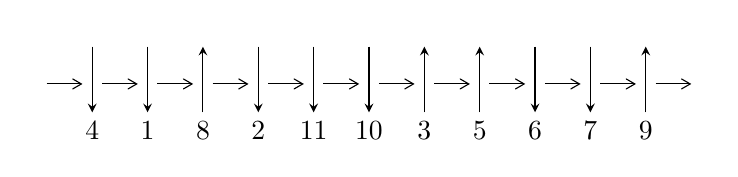
\begin{tikzpicture}[x=20pt, y=17pt]
	% nodes
	\node (C0) at (0, 0) {};
	\node (C1) at (1, 0) {};
	\node (C1U) at (1, +1) {};
	\node (C1D) at (1, -1) {4};

	\node (C2) at (2, 0) {};
	\node (C2U) at (2, +1) {};
	\node (C2D) at (2, -1) {1};

	\node (C3) at (3, 0) {};
	\node (C3U) at (3, +1) {};
	\node (C3D) at (3, -1) {8};

	\node (C4) at (4, 0) {};
	\node (C4U) at (4, +1) {};
	\node (C4D) at (4, -1) {2};

	\node (C5) at (5, 0) {};
	\node (C5U) at (5, +1) {};
	\node (C5D) at (5, -1) {11};

	\node (C6) at (6, 0) {};
	\node (C6U) at (6, +1) {};
	\node (C6D) at (6, -1) {10};

	\node (C7) at (7, 0) {};
	\node (C7U) at (7, +1) {};
	\node (C7D) at (7, -1) {3};

	\node (C8) at (8, 0) {};
	\node (C8U) at (8, +1) {};
	\node (C8D) at (8, -1) {5};

	\node (C9) at (9, 0) {};
	\node (C9U) at (9, +1) {};
	\node (C9D) at (9, -1) {6};

	\node (C10) at (10, 0) {};
	\node (C10U) at (10, +1) {};
	\node (C10D) at (10, -1) {7};

	\node (C11) at (11, 0) {};
	\node (C11U) at (11, +1) {};
	\node (C11D) at (11, -1) {9};
	\node (C12) at (12, 0) {};

	% arrows
	\draw[->,>={angle 60}]
	(C0) edge (C1) (C1) edge (C2) (C2) edge (C3) (C3) edge (C4) (C4) edge (C5) (C5) edge (C6) (C6) edge (C7) (C7) edge (C8) (C8) edge (C9) (C9) edge (C10) (C10) edge (C11) (C11) edge (C12) ;	\draw[->,>=stealth]
	(C1U) edge (C1D) (C2U) edge (C2D) (C3D) edge (C3U) (C4U) edge (C4D) (C5U) edge (C5D) (C6U) edge (C6D) (C7D) edge (C7U) (C8D) edge (C8U) (C9U) edge (C9D) (C10U) edge (C10D) (C11D) edge (C11U) ;
	\end{tikzpicture} \\
\hhline{~~} \\& 
\textbf{Solving Sequence} \\ \cline{2-2} 
 &
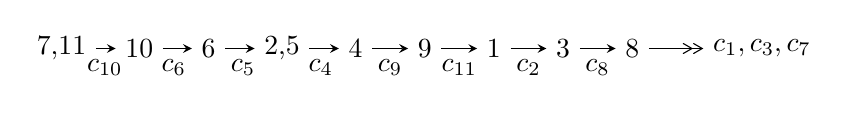
\begin{tikzpicture}[x=25pt, y=7pt]
	% node
	\node (A0) at (-1/8, 0) {7,11};
	\node (A1) at (1, 0) {10};
	\node (A2) at (2, 0) {6};
	\node (A3) at (49/16, 0) {2,5};
	\node (A4) at (33/8, 0) {4};
	\node (A5) at (41/8, 0) {9};
	\node (A6) at (49/8, 0) {1};
	\node (A7) at (57/8, 0) {3};
	\node (A8) at (65/8, 0) {8};
	\node (C1) at (1/2, -1) {$c_{10}$};
	\node (C2) at (3/2, -1) {$c_{6}$};
	\node (C3) at (5/2, -1) {$c_{5}$};
	\node (C4) at (29/8, -1) {$c_{4}$};
	\node (C5) at (37/8, -1) {$c_{9}$};
	\node (C6) at (45/8, -1) {$c_{11}$};
	\node (C7) at (53/8, -1) {$c_{2}$};
	\node (C8) at (61/8, -1) {$c_{8}$};
	\node (A9) at (10, 0) {$c_{1},c_{3},c_{7}$};

	% edge
	\draw[->,>=stealth]	
	(A0) edge (A1) (A1) edge (A2) (A2) edge (A3) (A3) edge (A4) (A4) edge (A5) (A5) edge (A6) (A6) edge (A7) (A7) edge (A8) ;
	\draw[->>,>={angle 60}]	
	(A8) edge (A9);
\end{tikzpicture} \\ 

\end{tabular} \\

\footnotetext{
The image of knot diagram is generated by the software ``\textbf{Draw programme}" developed by Andrew Bartholomew(\url{http://www.layer8.co.uk/maths/draw/index.htm\#Running-draw}), where we modified some parts for our purpose(\url{https://github.com/CATsTAILs/LinksPainter}).
}\phantom \\ \newline 
\centering \textbf{Ideals for irreducible components\footnotemark of $X_{\text{par}}$} 
 
\begin{align*}
I^u_{1}&=\langle 
- u^{63}- u^{62}+\cdots+b- u,\;u^{39}-18 u^{37}+\cdots-2 u^2+a,\;u^{64}+2 u^{63}+\cdots+u-1\rangle \\
I^u_{2}&=\langle 
b-1,\;- u^3+a+2 u,\;u^5- u^4-2 u^3+u^2+u+1\rangle \\
\\
\end{align*}
\raggedright * 2 irreducible components of $\dim_{\mathbb{C}}=0$, with total 69 representations.\\
\footnotetext{All coefficients of polynomials are rational numbers. But the coefficients are sometimes approximated in decimal forms when there is not enough margin.}
\newpage
\renewcommand{\arraystretch}{1}
\centering \section*{I. $I^u_{1}= \langle - u^{63}- u^{62}+\cdots+b- u,\;u^{39}-18 u^{37}+\cdots-2 u^2+a,\;u^{64}+2 u^{63}+\cdots+u-1 \rangle$}
\flushleft \textbf{(i) Arc colorings}\\
\begin{tabular}{m{7pt} m{180pt} m{7pt} m{180pt} }
\flushright $a_{7}=$&$\begin{pmatrix}0\\u\end{pmatrix}$ \\
\flushright $a_{11}=$&$\begin{pmatrix}1\\0\end{pmatrix}$ \\
\flushright $a_{10}=$&$\begin{pmatrix}1\\- u^2\end{pmatrix}$ \\
\flushright $a_{6}=$&$\begin{pmatrix}u\\- u^3+u\end{pmatrix}$ \\
\flushright $a_{2}=$&$\begin{pmatrix}- u^{39}+18 u^{37}+\cdots+6 u^3+2 u^2\\u^{63}+u^{62}+\cdots+u^2+u\end{pmatrix}$ \\
\flushright $a_{5}=$&$\begin{pmatrix}- u^3+2 u\\- u^3+u\end{pmatrix}$ \\
\flushright $a_{4}=$&$\begin{pmatrix}u^{63}+u^{62}+\cdots- u^2+2 u\\- u^{63}- u^{62}+\cdots- u^3- u\end{pmatrix}$ \\
\flushright $a_{9}=$&$\begin{pmatrix}- u^2+1\\u^4-2 u^2\end{pmatrix}$ \\
\flushright $a_{1}=$&$\begin{pmatrix}u^6-3 u^4+2 u^2+1\\- u^8+4 u^6-4 u^4\end{pmatrix}$ \\
\flushright $a_{3}=$&$\begin{pmatrix}u^{63}+u^{62}+\cdots- u-1\\u^{63}+u^{62}+\cdots+u^3+2 u^2\end{pmatrix}$ \\
\flushright $a_{8}=$&$\begin{pmatrix}- u^{10}+5 u^8-8 u^6+3 u^4+u^2+1\\- u^{10}+4 u^8-5 u^6+2 u^4- u^2\end{pmatrix}$\\ \flushright $a_{8}=$&$\begin{pmatrix}- u^{10}+5 u^8-8 u^6+3 u^4+u^2+1\\- u^{10}+4 u^8-5 u^6+2 u^4- u^2\end{pmatrix}$\\&\end{tabular}
\flushleft \textbf{(ii) Obstruction class $= -1$}\\~\\
\flushleft \textbf{(iii) Cusp Shapes $= -6 u^{63}-4 u^{62}+\cdots-13 u+2$}\\~\\
\newpage\renewcommand{\arraystretch}{1}
\flushleft \textbf{(iv) u-Polynomials at the component}\newline \\
\begin{tabular}{m{50pt}|m{274pt}}
Crossings & \hspace{64pt}u-Polynomials at each crossing \\
\hline $$\begin{aligned}c_{1},c_{4}\end{aligned}$$&$\begin{aligned}
&u^{64}-6 u^{63}+\cdots+3 u-1
\end{aligned}$\\
\hline $$\begin{aligned}c_{2}\end{aligned}$$&$\begin{aligned}
&u^{64}+30 u^{63}+\cdots+3 u+1
\end{aligned}$\\
\hline $$\begin{aligned}c_{3},c_{7}\end{aligned}$$&$\begin{aligned}
&u^{64}+u^{63}+\cdots+96 u+32
\end{aligned}$\\
\hline $$\begin{aligned}c_{5}\end{aligned}$$&$\begin{aligned}
&u^{64}-6 u^{63}+\cdots+5 u-1
\end{aligned}$\\
\hline $$\begin{aligned}c_{6},c_{9},c_{10}\end{aligned}$$&$\begin{aligned}
&u^{64}+2 u^{63}+\cdots+u-1
\end{aligned}$\\
\hline $$\begin{aligned}c_{8}\end{aligned}$$&$\begin{aligned}
&u^{64}-2 u^{63}+\cdots+8204 u-1960
\end{aligned}$\\
\hline $$\begin{aligned}c_{11}\end{aligned}$$&$\begin{aligned}
&u^{64}+14 u^{63}+\cdots+2787 u+207
\end{aligned}$\\
\hline
\end{tabular}\\~\\
\newpage\renewcommand{\arraystretch}{1}
\flushleft \textbf{(v) Riley Polynomials at the component}\newline \\
\begin{tabular}{m{50pt}|m{274pt}}
Crossings & \hspace{64pt}Riley Polynomials at each crossing \\
\hline $$\begin{aligned}c_{1},c_{4}\end{aligned}$$&$\begin{aligned}
&y^{64}-30 y^{63}+\cdots-3 y+1
\end{aligned}$\\
\hline $$\begin{aligned}c_{2}\end{aligned}$$&$\begin{aligned}
&y^{64}+14 y^{63}+\cdots+13 y+1
\end{aligned}$\\
\hline $$\begin{aligned}c_{3},c_{7}\end{aligned}$$&$\begin{aligned}
&y^{64}-33 y^{63}+\cdots-14848 y+1024
\end{aligned}$\\
\hline $$\begin{aligned}c_{5}\end{aligned}$$&$\begin{aligned}
&y^{64}-2 y^{63}+\cdots-9 y+1
\end{aligned}$\\
\hline $$\begin{aligned}c_{6},c_{9},c_{10}\end{aligned}$$&$\begin{aligned}
&y^{64}-58 y^{63}+\cdots- y+1
\end{aligned}$\\
\hline $$\begin{aligned}c_{8}\end{aligned}$$&$\begin{aligned}
&y^{64}-18 y^{63}+\cdots-40328176 y+3841600
\end{aligned}$\\
\hline $$\begin{aligned}c_{11}\end{aligned}$$&$\begin{aligned}
&y^{64}+18 y^{63}+\cdots+1021851 y+42849
\end{aligned}$\\
\hline
\end{tabular}\\~\\
\newpage\flushleft \textbf{(vi) Complex Volumes and Cusp Shapes}
$$\begin{array}{c|c|c}  
\text{Solutions to }I^u_{1}& \I (\text{vol} + \sqrt{-1}CS) & \text{Cusp shape}\\
 \hline 
\begin{aligned}
u &= \phantom{-}1.004890 + 0.212052 I \\
a &= \phantom{-}0.250176 - 1.256930 I \\
b &= -0.972468 + 0.330740 I\end{aligned}
 & \phantom{-}3.37131 - 1.86053 I & \phantom{-0.000000 } 0 \\ \hline\begin{aligned}
u &= \phantom{-}1.004890 - 0.212052 I \\
a &= \phantom{-}0.250176 + 1.256930 I \\
b &= -0.972468 - 0.330740 I\end{aligned}
 & \phantom{-}3.37131 + 1.86053 I & \phantom{-0.000000 } 0 \\ \hline\begin{aligned}
u &= -1.055590 + 0.097412 I \\
a &= \phantom{-}0.83771 - 1.53205 I \\
b &= -0.452362 + 0.922072 I\end{aligned}
 & -1.58334 + 2.05666 I & \phantom{-0.000000 } 0 \\ \hline\begin{aligned}
u &= -1.055590 - 0.097412 I \\
a &= \phantom{-}0.83771 + 1.53205 I \\
b &= -0.452362 - 0.922072 I\end{aligned}
 & -1.58334 - 2.05666 I & \phantom{-0.000000 } 0 \\ \hline\begin{aligned}
u &= \phantom{-}1.08657\phantom{ +0.000000I} \\
a &= \phantom{-}0.517514\phantom{ +0.000000I} \\
b &= \phantom{-}1.28011\phantom{ +0.000000I}\end{aligned}
 & -2.98700\phantom{ +0.000000I} & \phantom{-0.000000 } 0 \\ \hline\begin{aligned}
u &= \phantom{-}1.076070 + 0.243448 I \\
a &= \phantom{-}0.50549 + 1.44435 I \\
b &= \phantom{-}0.069484 - 0.831677 I\end{aligned}
 & \phantom{-}1.75966 - 7.47908 I & \phantom{-0.000000 } 0 \\ \hline\begin{aligned}
u &= \phantom{-}1.076070 - 0.243448 I \\
a &= \phantom{-}0.50549 - 1.44435 I \\
b &= \phantom{-}0.069484 + 0.831677 I\end{aligned}
 & \phantom{-}1.75966 + 7.47908 I & \phantom{-0.000000 } 0 \\ \hline\begin{aligned}
u &= \phantom{-}0.292951 + 0.725218 I \\
a &= -3.13866 + 0.47208 I \\
b &= -2.45175 + 0.82611 I\end{aligned}
 & \phantom{-}2.46662 - 11.29940 I & -1.16462 + 9.08913 I \\ \hline\begin{aligned}
u &= \phantom{-}0.292951 - 0.725218 I \\
a &= -3.13866 - 0.47208 I \\
b &= -2.45175 - 0.82611 I\end{aligned}
 & \phantom{-}2.46662 + 11.29940 I & -1.16462 - 9.08913 I \\ \hline\begin{aligned}
u &= \phantom{-}0.674453 + 0.386464 I \\
a &= -0.00066 - 2.55544 I \\
b &= -1.110180 - 0.550037 I\end{aligned}
 & \phantom{-}1.05339 + 7.31803 I & -3.59936 - 4.11166 I\\
 \hline 
 \end{array}$$\newpage$$\begin{array}{c|c|c}  
\text{Solutions to }I^u_{1}& \I (\text{vol} + \sqrt{-1}CS) & \text{Cusp shape}\\
 \hline 
\begin{aligned}
u &= \phantom{-}0.674453 - 0.386464 I \\
a &= -0.00066 + 2.55544 I \\
b &= -1.110180 + 0.550037 I\end{aligned}
 & \phantom{-}1.05339 - 7.31803 I & -3.59936 + 4.11166 I \\ \hline\begin{aligned}
u &= \phantom{-}0.705088 + 0.302401 I \\
a &= \phantom{-}0.83956 + 1.15317 I \\
b &= \phantom{-}0.077388 - 0.254328 I\end{aligned}
 & \phantom{-}3.02952 + 1.83201 I & -0.533486 + 0.085386 I \\ \hline\begin{aligned}
u &= \phantom{-}0.705088 - 0.302401 I \\
a &= \phantom{-}0.83956 - 1.15317 I \\
b &= \phantom{-}0.077388 + 0.254328 I\end{aligned}
 & \phantom{-}3.02952 - 1.83201 I & -0.533486 - 0.085386 I \\ \hline\begin{aligned}
u &= \phantom{-}0.265999 + 0.717941 I \\
a &= \phantom{-}1.40926 + 0.47850 I \\
b &= \phantom{-}1.178360 + 0.621823 I\end{aligned}
 & \phantom{-}4.64833 - 5.64259 I & \phantom{-}2.08406 + 5.05177 I \\ \hline\begin{aligned}
u &= \phantom{-}0.265999 - 0.717941 I \\
a &= \phantom{-}1.40926 - 0.47850 I \\
b &= \phantom{-}1.178360 - 0.621823 I\end{aligned}
 & \phantom{-}4.64833 + 5.64259 I & \phantom{-}2.08406 - 5.05177 I \\ \hline\begin{aligned}
u &= -0.268310 + 0.684190 I \\
a &= -3.11925 - 1.34879 I \\
b &= -2.29400 - 1.31119 I\end{aligned}
 & -0.18871 + 5.19299 I & -2.32409 - 6.82469 I \\ \hline\begin{aligned}
u &= -0.268310 - 0.684190 I \\
a &= -3.11925 + 1.34879 I \\
b &= -2.29400 + 1.31119 I\end{aligned}
 & -0.18871 - 5.19299 I & -2.32409 + 6.82469 I \\ \hline\begin{aligned}
u &= \phantom{-}0.166461 + 0.708672 I \\
a &= -1.78632 + 0.78559 I \\
b &= -1.57846 + 0.71331 I\end{aligned}
 & \phantom{-}5.88443 - 1.71228 I & \phantom{-}4.06856 + 3.31380 I \\ \hline\begin{aligned}
u &= \phantom{-}0.166461 - 0.708672 I \\
a &= -1.78632 - 0.78559 I \\
b &= -1.57846 - 0.71331 I\end{aligned}
 & \phantom{-}5.88443 + 1.71228 I & \phantom{-}4.06856 - 3.31380 I \\ \hline\begin{aligned}
u &= -1.27342\phantom{ +0.000000I} \\
a &= \phantom{-}0.512497\phantom{ +0.000000I} \\
b &= -0.111947\phantom{ +0.000000I}\end{aligned}
 & -2.82174\phantom{ +0.000000I} & \phantom{-0.000000 } 0\\
 \hline 
 \end{array}$$\newpage$$\begin{array}{c|c|c}  
\text{Solutions to }I^u_{1}& \I (\text{vol} + \sqrt{-1}CS) & \text{Cusp shape}\\
 \hline 
\begin{aligned}
u &= -0.379910 + 0.618311 I \\
a &= \phantom{-}0.888593 - 0.950785 I \\
b &= \phantom{-}0.785579 + 0.082329 I\end{aligned}
 & -1.309430 + 0.220190 I & -2.16669 + 0.94520 I \\ \hline\begin{aligned}
u &= -0.379910 - 0.618311 I \\
a &= \phantom{-}0.888593 + 0.950785 I \\
b &= \phantom{-}0.785579 - 0.082329 I\end{aligned}
 & -1.309430 - 0.220190 I & -2.16669 - 0.94520 I \\ \hline\begin{aligned}
u &= \phantom{-}0.116871 + 0.709884 I \\
a &= \phantom{-}1.79401 - 0.11144 I \\
b &= \phantom{-}1.312960 + 0.524885 I\end{aligned}
 & \phantom{-}4.64291 + 3.88634 I & \phantom{-}2.43594 - 2.51707 I \\ \hline\begin{aligned}
u &= \phantom{-}0.116871 - 0.709884 I \\
a &= \phantom{-}1.79401 + 0.11144 I \\
b &= \phantom{-}1.312960 - 0.524885 I\end{aligned}
 & \phantom{-}4.64291 - 3.88634 I & \phantom{-}2.43594 + 2.51707 I \\ \hline\begin{aligned}
u &= -0.460178 + 0.533945 I \\
a &= \phantom{-}0.637038 - 0.795810 I \\
b &= \phantom{-}1.111230 - 0.236500 I\end{aligned}
 & -1.65255 + 3.56868 I & -3.94595 - 7.64427 I \\ \hline\begin{aligned}
u &= -0.460178 - 0.533945 I \\
a &= \phantom{-}0.637038 + 0.795810 I \\
b &= \phantom{-}1.111230 + 0.236500 I\end{aligned}
 & -1.65255 - 3.56868 I & -3.94595 + 7.64427 I \\ \hline\begin{aligned}
u &= \phantom{-}0.259055 + 0.653388 I \\
a &= \phantom{-}1.06464 + 0.97600 I \\
b &= \phantom{-}0.990905 - 0.182467 I\end{aligned}
 & -1.20405 - 2.76775 I & -0.87874 + 6.15771 I \\ \hline\begin{aligned}
u &= \phantom{-}0.259055 - 0.653388 I \\
a &= \phantom{-}1.06464 - 0.97600 I \\
b &= \phantom{-}0.990905 + 0.182467 I\end{aligned}
 & -1.20405 + 2.76775 I & -0.87874 - 6.15771 I \\ \hline\begin{aligned}
u &= -0.204298 + 0.641678 I \\
a &= \phantom{-}2.07861 - 0.64563 I \\
b &= \phantom{-}1.34976 - 0.78269 I\end{aligned}
 & \phantom{-}0.748257 + 0.939190 I & \phantom{-}0.11212 - 1.46039 I \\ \hline\begin{aligned}
u &= -0.204298 - 0.641678 I \\
a &= \phantom{-}2.07861 + 0.64563 I \\
b &= \phantom{-}1.34976 + 0.78269 I\end{aligned}
 & \phantom{-}0.748257 - 0.939190 I & \phantom{-}0.11212 + 1.46039 I\\
 \hline 
 \end{array}$$\newpage$$\begin{array}{c|c|c}  
\text{Solutions to }I^u_{1}& \I (\text{vol} + \sqrt{-1}CS) & \text{Cusp shape}\\
 \hline 
\begin{aligned}
u &= -1.319680 + 0.270463 I \\
a &= \phantom{-}0.628923 - 0.555572 I \\
b &= \phantom{-}2.00427 + 0.11792 I\end{aligned}
 & \phantom{-}0.150980 - 0.347116 I & \phantom{-0.000000 } 0 \\ \hline\begin{aligned}
u &= -1.319680 - 0.270463 I \\
a &= \phantom{-}0.628923 + 0.555572 I \\
b &= \phantom{-}2.00427 - 0.11792 I\end{aligned}
 & \phantom{-}0.150980 + 0.347116 I & \phantom{-0.000000 } 0 \\ \hline\begin{aligned}
u &= -1.353850 + 0.278392 I \\
a &= -0.922498 + 0.572074 I \\
b &= -1.59733 - 1.65323 I\end{aligned}
 & \phantom{-}1.08775 + 5.28117 I & \phantom{-0.000000 } 0 \\ \hline\begin{aligned}
u &= -1.353850 - 0.278392 I \\
a &= -0.922498 - 0.572074 I \\
b &= -1.59733 + 1.65323 I\end{aligned}
 & \phantom{-}1.08775 - 5.28117 I & \phantom{-0.000000 } 0 \\ \hline\begin{aligned}
u &= -0.556271 + 0.257738 I \\
a &= \phantom{-}1.06140 + 2.71158 I \\
b &= -0.484179 + 0.678880 I\end{aligned}
 & -1.60289 - 1.70495 I & -6.10429 + 1.65168 I \\ \hline\begin{aligned}
u &= -0.556271 - 0.257738 I \\
a &= \phantom{-}1.06140 - 2.71158 I \\
b &= -0.484179 - 0.678880 I\end{aligned}
 & -1.60289 + 1.70495 I & -6.10429 - 1.65168 I \\ \hline\begin{aligned}
u &= \phantom{-}1.387450 + 0.186851 I \\
a &= -0.335032 + 0.455289 I \\
b &= \phantom{-}0.124901 + 1.401000 I\end{aligned}
 & -5.22435 - 3.56448 I & \phantom{-0.000000 } 0 \\ \hline\begin{aligned}
u &= \phantom{-}1.387450 - 0.186851 I \\
a &= -0.335032 - 0.455289 I \\
b &= \phantom{-}0.124901 - 1.401000 I\end{aligned}
 & -5.22435 + 3.56448 I & \phantom{-0.000000 } 0 \\ \hline\begin{aligned}
u &= \phantom{-}1.384430 + 0.250118 I \\
a &= \phantom{-}0.470700 + 0.975593 I \\
b &= \phantom{-}2.41332 + 0.37758 I\end{aligned}
 & -4.32280 - 4.18388 I & \phantom{-0.000000 } 0 \\ \hline\begin{aligned}
u &= \phantom{-}1.384430 - 0.250118 I \\
a &= \phantom{-}0.470700 - 0.975593 I \\
b &= \phantom{-}2.41332 - 0.37758 I\end{aligned}
 & -4.32280 + 4.18388 I & \phantom{-0.000000 } 0\\
 \hline 
 \end{array}$$\newpage$$\begin{array}{c|c|c}  
\text{Solutions to }I^u_{1}& \I (\text{vol} + \sqrt{-1}CS) & \text{Cusp shape}\\
 \hline 
\begin{aligned}
u &= -1.410150 + 0.091621 I \\
a &= \phantom{-}0.171722 - 0.446103 I \\
b &= -0.051337 - 0.869147 I\end{aligned}
 & -3.31779 - 0.73149 I & \phantom{-0.000000 } 0 \\ \hline\begin{aligned}
u &= -1.410150 - 0.091621 I \\
a &= \phantom{-}0.171722 + 0.446103 I \\
b &= -0.051337 + 0.869147 I\end{aligned}
 & -3.31779 + 0.73149 I & \phantom{-0.000000 } 0 \\ \hline\begin{aligned}
u &= -1.404660 + 0.156512 I \\
a &= -0.481712 - 0.823798 I \\
b &= \phantom{-}1.44039 + 0.27511 I\end{aligned}
 & -7.96725 + 2.25757 I & \phantom{-0.000000 } 0 \\ \hline\begin{aligned}
u &= -1.404660 - 0.156512 I \\
a &= -0.481712 + 0.823798 I \\
b &= \phantom{-}1.44039 - 0.27511 I\end{aligned}
 & -7.96725 - 2.25757 I & \phantom{-0.000000 } 0 \\ \hline\begin{aligned}
u &= \phantom{-}1.407530 + 0.132731 I \\
a &= \phantom{-}1.36353 - 0.57844 I \\
b &= \phantom{-}0.66427 - 2.25478 I\end{aligned}
 & -7.47816 + 0.17720 I & \phantom{-0.000000 } 0 \\ \hline\begin{aligned}
u &= \phantom{-}1.407530 - 0.132731 I \\
a &= \phantom{-}1.36353 + 0.57844 I \\
b &= \phantom{-}0.66427 + 2.25478 I\end{aligned}
 & -7.47816 - 0.17720 I & \phantom{-0.000000 } 0 \\ \hline\begin{aligned}
u &= -1.40289 + 0.25793 I \\
a &= -0.099708 - 0.974841 I \\
b &= \phantom{-}0.717554 + 0.201107 I\end{aligned}
 & -6.51086 + 6.10114 I & \phantom{-0.000000 } 0 \\ \hline\begin{aligned}
u &= -1.40289 - 0.25793 I \\
a &= -0.099708 + 0.974841 I \\
b &= \phantom{-}0.717554 - 0.201107 I\end{aligned}
 & -6.51086 - 6.10114 I & \phantom{-0.000000 } 0 \\ \hline\begin{aligned}
u &= \phantom{-}1.40734 + 0.26932 I \\
a &= -1.68136 - 0.99882 I \\
b &= -2.91941 + 2.36420 I\end{aligned}
 & -5.53651 - 8.66838 I & \phantom{-0.000000 } 0 \\ \hline\begin{aligned}
u &= \phantom{-}1.40734 - 0.26932 I \\
a &= -1.68136 + 0.99882 I \\
b &= -2.91941 - 2.36420 I\end{aligned}
 & -5.53651 + 8.66838 I & \phantom{-0.000000 } 0\\
 \hline 
 \end{array}$$\newpage$$\begin{array}{c|c|c}  
\text{Solutions to }I^u_{1}& \I (\text{vol} + \sqrt{-1}CS) & \text{Cusp shape}\\
 \hline 
\begin{aligned}
u &= -1.40814 + 0.28394 I \\
a &= \phantom{-}0.280476 - 0.719527 I \\
b &= \phantom{-}1.97690 - 0.33914 I\end{aligned}
 & -0.68966 + 9.28326 I & \phantom{-0.000000 } 0 \\ \hline\begin{aligned}
u &= -1.40814 - 0.28394 I \\
a &= \phantom{-}0.280476 + 0.719527 I \\
b &= \phantom{-}1.97690 + 0.33914 I\end{aligned}
 & -0.68966 - 9.28326 I & \phantom{-0.000000 } 0 \\ \hline\begin{aligned}
u &= -1.42115 + 0.28534 I \\
a &= -1.34480 + 1.32214 I \\
b &= -3.09851 - 1.54301 I\end{aligned}
 & -3.0092 + 14.9742 I & \phantom{-0.000000 } 0 \\ \hline\begin{aligned}
u &= -1.42115 - 0.28534 I \\
a &= -1.34480 - 1.32214 I \\
b &= -3.09851 + 1.54301 I\end{aligned}
 & -3.0092 - 14.9742 I & \phantom{-0.000000 } 0 \\ \hline\begin{aligned}
u &= -1.44601 + 0.10453 I \\
a &= \phantom{-}0.955221 + 0.877194 I \\
b &= -0.16080 + 1.87965 I\end{aligned}
 & -5.55732 - 5.80431 I & \phantom{-0.000000 } 0 \\ \hline\begin{aligned}
u &= -1.44601 - 0.10453 I \\
a &= \phantom{-}0.955221 - 0.877194 I \\
b &= -0.16080 - 1.87965 I\end{aligned}
 & -5.55732 + 5.80431 I & \phantom{-0.000000 } 0 \\ \hline\begin{aligned}
u &= \phantom{-}1.44004 + 0.23244 I \\
a &= -0.095745 + 0.853500 I \\
b &= \phantom{-}0.714563 + 0.171726 I\end{aligned}
 & -7.13968 - 3.33308 I & \phantom{-0.000000 } 0 \\ \hline\begin{aligned}
u &= \phantom{-}1.44004 - 0.23244 I \\
a &= -0.095745 - 0.853500 I \\
b &= \phantom{-}0.714563 - 0.171726 I\end{aligned}
 & -7.13968 + 3.33308 I & \phantom{-0.000000 } 0 \\ \hline\begin{aligned}
u &= \phantom{-}1.44782 + 0.18947 I \\
a &= -0.258808 + 0.695694 I \\
b &= \phantom{-}1.43274 + 0.05713 I\end{aligned}
 & -7.74951 - 6.19199 I & \phantom{-0.000000 } 0 \\ \hline\begin{aligned}
u &= \phantom{-}1.44782 - 0.18947 I \\
a &= -0.258808 - 0.695694 I \\
b &= \phantom{-}1.43274 - 0.05713 I\end{aligned}
 & -7.74951 + 6.19199 I & \phantom{-0.000000 } 0\\
 \hline 
 \end{array}$$\newpage$$\begin{array}{c|c|c}  
\text{Solutions to }I^u_{1}& \I (\text{vol} + \sqrt{-1}CS) & \text{Cusp shape}\\
 \hline 
\begin{aligned}
u &= -0.234891 + 0.464221 I \\
a &= \phantom{-}0.496892 - 0.920682 I \\
b &= \phantom{-}0.051241 - 0.444007 I\end{aligned}
 & -0.038168 + 1.118320 I & -0.73760 - 6.33469 I \\ \hline\begin{aligned}
u &= -0.234891 - 0.464221 I \\
a &= \phantom{-}0.496892 + 0.920682 I \\
b &= \phantom{-}0.051241 + 0.444007 I\end{aligned}
 & -0.038168 - 1.118320 I & -0.73760 + 6.33469 I \\ \hline\begin{aligned}
u &= \phantom{-}0.382966 + 0.305636 I \\
a &= \phantom{-}0.015592 + 1.148670 I \\
b &= \phantom{-}1.170900 + 0.079635 I\end{aligned}
 & -2.38212 - 0.33638 I & -5.62748 - 1.67456 I \\ \hline\begin{aligned}
u &= \phantom{-}0.382966 - 0.305636 I \\
a &= \phantom{-}0.015592 - 1.148670 I \\
b &= \phantom{-}1.170900 - 0.079635 I\end{aligned}
 & -2.38212 + 0.33638 I & -5.62748 + 1.67456 I\\
 \hline 
 \end{array}$$\newpage\newpage\renewcommand{\arraystretch}{1}
\centering \section*{II. $I^u_{2}= \langle b-1,\;- u^3+a+2 u,\;u^5- u^4-2 u^3+u^2+u+1 \rangle$}
\flushleft \textbf{(i) Arc colorings}\\
\begin{tabular}{m{7pt} m{180pt} m{7pt} m{180pt} }
\flushright $a_{7}=$&$\begin{pmatrix}0\\u\end{pmatrix}$ \\
\flushright $a_{11}=$&$\begin{pmatrix}1\\0\end{pmatrix}$ \\
\flushright $a_{10}=$&$\begin{pmatrix}1\\- u^2\end{pmatrix}$ \\
\flushright $a_{6}=$&$\begin{pmatrix}u\\- u^3+u\end{pmatrix}$ \\
\flushright $a_{2}=$&$\begin{pmatrix}u^3-2 u\\1\end{pmatrix}$ \\
\flushright $a_{5}=$&$\begin{pmatrix}- u^3+2 u\\- u^3+u\end{pmatrix}$ \\
\flushright $a_{4}=$&$\begin{pmatrix}0\\- u^3+u+1\end{pmatrix}$ \\
\flushright $a_{9}=$&$\begin{pmatrix}- u^2+1\\u^4-2 u^2\end{pmatrix}$ \\
\flushright $a_{1}=$&$\begin{pmatrix}u^3-2 u\\u^3- u\end{pmatrix}$ \\
\flushright $a_{3}=$&$\begin{pmatrix}0\\- u^3+u+1\end{pmatrix}$ \\
\flushright $a_{8}=$&$\begin{pmatrix}0\\u\end{pmatrix}$\\ \flushright $a_{8}=$&$\begin{pmatrix}0\\u\end{pmatrix}$\\&\end{tabular}
\flushleft \textbf{(ii) Obstruction class $= 1$}\\~\\
\flushleft \textbf{(iii) Cusp Shapes $= 5 u^3- u^2-8 u-9$}\\~\\
\newpage\renewcommand{\arraystretch}{1}
\flushleft \textbf{(iv) u-Polynomials at the component}\newline \\
\begin{tabular}{m{50pt}|m{274pt}}
Crossings & \hspace{64pt}u-Polynomials at each crossing \\
\hline $$\begin{aligned}c_{1}\end{aligned}$$&$\begin{aligned}
&(u-1)^5
\end{aligned}$\\
\hline $$\begin{aligned}c_{2},c_{4}\end{aligned}$$&$\begin{aligned}
&(u+1)^5
\end{aligned}$\\
\hline $$\begin{aligned}c_{3},c_{7}\end{aligned}$$&$\begin{aligned}
&u^5
\end{aligned}$\\
\hline $$\begin{aligned}c_{5}\end{aligned}$$&$\begin{aligned}
&u^5-3 u^4+4 u^3- u^2- u+1
\end{aligned}$\\
\hline $$\begin{aligned}c_{6}\end{aligned}$$&$\begin{aligned}
&u^5+u^4-2 u^3- u^2+u-1
\end{aligned}$\\
\hline $$\begin{aligned}c_{8},c_{11}\end{aligned}$$&$\begin{aligned}
&u^5+u^4+2 u^3+u^2+u+1
\end{aligned}$\\
\hline $$\begin{aligned}c_{9},c_{10}\end{aligned}$$&$\begin{aligned}
&u^5- u^4-2 u^3+u^2+u+1
\end{aligned}$\\
\hline
\end{tabular}\\~\\
\newpage\renewcommand{\arraystretch}{1}
\flushleft \textbf{(v) Riley Polynomials at the component}\newline \\
\begin{tabular}{m{50pt}|m{274pt}}
Crossings & \hspace{64pt}Riley Polynomials at each crossing \\
\hline $$\begin{aligned}c_{1},c_{2},c_{4}\end{aligned}$$&$\begin{aligned}
&(y-1)^5
\end{aligned}$\\
\hline $$\begin{aligned}c_{3},c_{7}\end{aligned}$$&$\begin{aligned}
&y^5
\end{aligned}$\\
\hline $$\begin{aligned}c_{5}\end{aligned}$$&$\begin{aligned}
&y^5- y^4+8 y^3-3 y^2+3 y-1
\end{aligned}$\\
\hline $$\begin{aligned}c_{6},c_{9},c_{10}\end{aligned}$$&$\begin{aligned}
&y^5-5 y^4+8 y^3-3 y^2- y-1
\end{aligned}$\\
\hline $$\begin{aligned}c_{8},c_{11}\end{aligned}$$&$\begin{aligned}
&y^5+3 y^4+4 y^3+y^2- y-1
\end{aligned}$\\
\hline
\end{tabular}\\~\\
\newpage\flushleft \textbf{(vi) Complex Volumes and Cusp Shapes}
$$\begin{array}{c|c|c}  
\text{Solutions to }I^u_{2}& \I (\text{vol} + \sqrt{-1}CS) & \text{Cusp shape}\\
 \hline 
\begin{aligned}
u &= -1.21774\phantom{ +0.000000I} \\
a &= \phantom{-}0.629714\phantom{ +0.000000I} \\
b &= \phantom{-}1.00000\phantom{ +0.000000I}\end{aligned}
 & -4.04602\phantom{ +0.000000I} & -9.76980\phantom{ +0.000000I} \\ \hline\begin{aligned}
u &= -0.309916 + 0.549911 I \\
a &= \phantom{-}0.871221 - 1.107660 I \\
b &= \phantom{-}1.00000\phantom{ +0.000000I}\end{aligned}
 & -1.97403 + 1.53058 I & -5.05737 - 4.09764 I \\ \hline\begin{aligned}
u &= -0.309916 - 0.549911 I \\
a &= \phantom{-}0.871221 + 1.107660 I \\
b &= \phantom{-}1.00000\phantom{ +0.000000I}\end{aligned}
 & -1.97403 - 1.53058 I & -5.05737 + 4.09764 I \\ \hline\begin{aligned}
u &= \phantom{-}1.41878 + 0.21917 I \\
a &= -0.186078 + 0.874646 I \\
b &= \phantom{-}1.00000\phantom{ +0.000000I}\end{aligned}
 & -7.51750 - 4.40083 I & -9.05774 + 4.18967 I \\ \hline\begin{aligned}
u &= \phantom{-}1.41878 - 0.21917 I \\
a &= -0.186078 - 0.874646 I \\
b &= \phantom{-}1.00000\phantom{ +0.000000I}\end{aligned}
 & -7.51750 + 4.40083 I & -9.05774 - 4.18967 I\\
 \hline 
 \end{array}$$\newpage
\newpage\renewcommand{\arraystretch}{1}
\centering \section*{ III. u-Polynomials}
\begin{tabular}{m{50pt}|m{274pt}}
Crossings & \hspace{64pt}u-Polynomials at each crossing \\
\hline $$\begin{aligned}c_{1}\end{aligned}$$&$\begin{aligned}
&((u-1)^5)(u^{64}-6 u^{63}+\cdots+3 u-1)
\end{aligned}$\\
\hline $$\begin{aligned}c_{2}\end{aligned}$$&$\begin{aligned}
&((u+1)^5)(u^{64}+30 u^{63}+\cdots+3 u+1)
\end{aligned}$\\
\hline $$\begin{aligned}c_{3},c_{7}\end{aligned}$$&$\begin{aligned}
&u^5(u^{64}+u^{63}+\cdots+96 u+32)
\end{aligned}$\\
\hline $$\begin{aligned}c_{4}\end{aligned}$$&$\begin{aligned}
&((u+1)^5)(u^{64}-6 u^{63}+\cdots+3 u-1)
\end{aligned}$\\
\hline $$\begin{aligned}c_{5}\end{aligned}$$&$\begin{aligned}
&(u^5-3 u^4+4 u^3- u^2- u+1)(u^{64}-6 u^{63}+\cdots+5 u-1)
\end{aligned}$\\
\hline $$\begin{aligned}c_{6}\end{aligned}$$&$\begin{aligned}
&(u^5+u^4-2 u^3- u^2+u-1)(u^{64}+2 u^{63}+\cdots+u-1)
\end{aligned}$\\
\hline $$\begin{aligned}c_{8}\end{aligned}$$&$\begin{aligned}
&(u^5+u^4+2 u^3+u^2+u+1)(u^{64}-2 u^{63}+\cdots+8204 u-1960)
\end{aligned}$\\
\hline $$\begin{aligned}c_{9},c_{10}\end{aligned}$$&$\begin{aligned}
&(u^5- u^4-2 u^3+u^2+u+1)(u^{64}+2 u^{63}+\cdots+u-1)
\end{aligned}$\\
\hline $$\begin{aligned}c_{11}\end{aligned}$$&$\begin{aligned}
&(u^5+u^4+2 u^3+u^2+u+1)(u^{64}+14 u^{63}+\cdots+2787 u+207)
\end{aligned}$\\
\hline
\end{tabular}\newpage\renewcommand{\arraystretch}{1}
\centering \section*{ IV. Riley Polynomials}
\begin{tabular}{m{50pt}|m{274pt}}
Crossings & \hspace{64pt}Riley Polynomials at each crossing \\
\hline $$\begin{aligned}c_{1},c_{4}\end{aligned}$$&$\begin{aligned}
&((y-1)^5)(y^{64}-30 y^{63}+\cdots-3 y+1)
\end{aligned}$\\
\hline $$\begin{aligned}c_{2}\end{aligned}$$&$\begin{aligned}
&((y-1)^5)(y^{64}+14 y^{63}+\cdots+13 y+1)
\end{aligned}$\\
\hline $$\begin{aligned}c_{3},c_{7}\end{aligned}$$&$\begin{aligned}
&y^5(y^{64}-33 y^{63}+\cdots-14848 y+1024)
\end{aligned}$\\
\hline $$\begin{aligned}c_{5}\end{aligned}$$&$\begin{aligned}
&(y^5- y^4+8 y^3-3 y^2+3 y-1)(y^{64}-2 y^{63}+\cdots-9 y+1)
\end{aligned}$\\
\hline $$\begin{aligned}c_{6},c_{9},c_{10}\end{aligned}$$&$\begin{aligned}
&(y^5-5 y^4+8 y^3-3 y^2- y-1)(y^{64}-58 y^{63}+\cdots- y+1)
\end{aligned}$\\
\hline $$\begin{aligned}c_{8}\end{aligned}$$&$\begin{aligned}
&(y^5+3 y^4+4 y^3+y^2- y-1)\\
&\cdot(y^{64}-18 y^{63}+\cdots-40328176 y+3841600)
\end{aligned}$\\
\hline $$\begin{aligned}c_{11}\end{aligned}$$&$\begin{aligned}
&(y^5+3 y^4+4 y^3+y^2- y-1)(y^{64}+18 y^{63}+\cdots+1021851 y+42849)
\end{aligned}$\\
\hline
\end{tabular}
\vskip 2pc
\end{document}